\documentclass[sigplan,9pt]{acmart}
\usepackage[latin9]{inputenc}
%\setcounter{secnumdepth}{2}
%\setcounter{tocdepth}{2}

\usepackage[english]{babel}
\usepackage{graphicx}
\usepackage{url}
\usepackage{natbib}
\usepackage{caption}
\usepackage{subcaption}
\usepackage{listings}
\usepackage{amsthm}
\usepackage{subfiles}
\usepackage{float}
%\usepackage{hyperref}

\newtheorem*{slo}{SLO}

% Tenslotte wordt hyperref gebruikt voor pdf bestanden.
% Dit mag verwijderd worden voor de af te drukken versie.
%\usepackage[pdfusetitle,colorlinks,plainpages=false]{hyperref}


\newcommand*\circled[1]{\tikz[baseline=(char.base)]{
            \node[shape=circle,fill,inner sep=0.4pt] (char) {\textcolor{white}{#1}};}}


% Rights management information. 
% This information is sent to you when you complete the rights form.
% These commands have SAMPLE values in them; it is your responsibility as an author to replace
% the commands and values with those provided to you when you complete the rights form.
%
% These commands are for a PROCEEDINGS abstract or paper.
\copyrightyear{2019}
\acmYear{2019}
\setcopyright{acmlicensed}
\acmConference[Middleware~'19]{Middleware '19}{December 09--13, 2019}{UC Davis, CA, USA}
\acmBooktitle{Middleware '19, December 09--13, 2019, UC Davis, CA, USA}
\acmPrice{15.00}
\acmDOI{}
\settopmatter{printfolios=true,printacmref=false,printccs=false}
\renewcommand\footnotetextcopyrightpermission[1]{} % removes footnote with conference information in first column

%\newwatermark[allpages,color=red!50,angle=45,scale=1,xpos=0,ypos=0]{Confidential version available to Joerg Domaschka and Daniel Seybold}

% switch to key style at EOL
%\lst@AddToHook{EveryLine}{\ifx\lst@language\language@yaml\YAMLkeystyle\fi}
%\makeatother

%\newcommand\ProcessThreeDashes{\llap{\color{cyan}\mdseries-{-}-}}


%\urlstyle{sf} 
%\sloppy

\keywords{Auto-scaling, Adaptive resource management, Container orchestration frameworks}

\begin{CCSXML}
<ccs2012>
<concept>
<concept_id>10011007.10010940.10011003.10011002</concept_id>
<concept_desc>Software and its engineering~Software performance</concept_desc>
<concept_significance>500</concept_significance>
</concept>
<concept>
<concept_id>10011007.10010940.10010971.10011120.10003100</concept_id>
<concept_desc>Software and its engineering~Cloud computing</concept_desc>
<concept_significance>300</concept_significance>
</concept>
<concept>
<concept_id>10011007.10011006.10011066.10011068</concept_id>
<concept_desc>Software and its engineering~Software as a service orchestration system</concept_desc>
<concept_significance>300</concept_significance>
</concept>
</ccs2012>
\end{CCSXML}

\ccsdesc[500]{Software and its engineering~Software performance}
\ccsdesc[300]{Software and its engineering~Cloud computing}
\ccsdesc[300]{Software and its engineering~Software as a service orchestration system}



\begin{document}

\title{Leveraging Kubernetes for adaptive and cost-efficient resource management}
%\renewcommand{\shorttitle}{A framework for black-box SLO tuning in Kubernetes}

\author{Stef Verreydt, Emad Heydari Beni, Eddy Truyen, Bert Lagaisse, Wouter Joosen}
\affiliation{\textit{imec-DistriNet, KU Leuven, Belgium}}
\email{firstname.lastname@cs.kuleuven.be}
\renewcommand{\shortauthors}{S. Verreydt et al.}

\begin{abstract}
Software providers face the challenge of minimizing the amount of resources used while still meeting their customer's requirements. Several frameworks to manage resources and applications in a distributed environment are available, but their development is still ongoing and the state of the art is rapidly evolving, making it a challenge to use such frameworks and their features effectively in practice. The goal of this paper is to research how applications can be enhanced with adaptive performance management by relying on the capabilities of Kubernetes, a popular framework for container orchestration. In particular, horizontal as well as vertical scaling concepts of Kubernetes may prove useful to support adaptive resource allocation. Moreover, concepts for oversubscription as a way to simulate vertical scaling without having to reschedule applications, will be evaluated. Through a series of experiments involving multiple applications and workloads, the effects of different configurations and combinations of horizontal and vertical scaling in Kubernetes are explored. Both the resource utilization of the nodes and the applications' performance are taken into account. In brief, the resource management concepts of Kubernetes allow to simulate vertical scaling without a negative effect on performance. The effectiveness of the default horizontal autoscaler, however, depends on the type of application and the user workload at hand.
\end{abstract}

\maketitle


\section{Introduction}
\label{chap:introduction}
Companies tend to move their resources to the cloud rather than keeping them on their own infrastructure as it offers numerous advantages (i.e.~\citep{AhmadiM.2018Caao}). SaaS providers aim to provide their services as cost-efficiently as possible. In this regard, they face the continuous challenge of utilizing only a minimal amount of resources while still meeting their customers' requirements. One way to reduce the amount of resources needed is by locating multiple applications on the same node. This entails new challenges, e.g., determining how to divide over-provisioned resources among the deployed applications, and how to handle resource contention in general. 

Kubernetes is a popular open source framework for managing containerized applications in a distributed environment, providing basic mechanisms for deployment, maintenance and scaling of applications~\citep{kubernetes_github}. It also offers several useful features for resource management. 
A pod in Kubernetes is the smallest deployable unit of computing which can be created and managed~\citep{pod}. Containers belonging to the same application are grouped together in pods. 
The resources used by a pod can be limited, e.g., by setting its so-called requests and limits. The request is the amount of resources which it is guaranteed to get; the limit is the maximal amount of resources it can obtain~\citep{requestlimit}. When there is resource contention in a node, the resources are divided among the pods according to the relative weight of their requests. This mechanism is reffered to as \textit{cpu-shares}. Another way of adjusting the resources available to an application is to scale it. Kubernetes offers default horizontal and vertical autoscalers, called the Horizontal Pod Autoscaler (HPA) and Vertical Pod Autoscaler (VPA) respectively. However, a well-known disadvantage of the VPA is that it currently requires to reschedule Pods when dynamically adjusting requests or limits ~\citep{in-place-pod-resources-updates}.%\footnote{although, a design proposal to resolve this issue is being discussed~\citep{in-place-pod-resources-updates}}.

%So far, research on resource management in container-based environments has been rather scarce, as it is still relatively new compared to VM-based environments~\citep{Al-DhuraibiYahya2018EiCC}~\citep{CoutinhoEmanuel2015Eicc}. 
Kubernetes is evolving rapidly. Meanwhile, both documentation and research are struggling to keep up with its development, especially since most research is aimed towards custom scaling techniques (e.g.,~\citep{hyscale}~\citep{caravel}). The Kubernetes mechanisms are poorly documented, which hampers effective use. Multiple questions may arise when configuring a Kubernetes cluster, e.g., how to choose suitable requests and limits, on which nodes to locate certain pods and how to configure an autoscaler. 
The goal of this paper is therefore to research how different Kubernetes features can be leveraged to cost-effectively manage resources in the framework while also meeting SLOs in the presence of dynamically evolving workloads. More concretely, we aim to provide answers to the following questions:
\setlist{nolistsep}
\begin{itemize}[noitemsep]
    \itemsep0em 
    \item What is the impact of different request and limit configurations?
    \item Does co-locating a high priority pod with a low priority pod affect the performance of the high priority pod?
    \item What is the performance impact of scaling an application using the HPA?
\end{itemize}

Different configurations may result in different performance gains (or losses) depending on the environment. For example, the user load may be very bursty, in which case using the oversubscription concepts or the HPA may not always lead to the expected results. Hence, the aforementioned impacts of the different mechanisms will be tested for both linearly increasing and bursty workloads. In this paper, however, only CPU intensive workloads will be examined. 
%Scaling memory bound systems is less common as performing a static optimization of needed memory often suffices. Furthermore, Kubernetes does not offer support for configuring network and disk resources. % candidate

% This paper evaluates the effects of simulating vertical scaling through the use of requests and limits and co-locating high-priority and low-priority pods, horizontal scaling using the default Kubernetes HPA, and a combination of both, in different environments. A test application deployed on a Kubernetes cluster is subjected to multiple experiments to illustrate the impact of different configurations.

% \begin{itemize}
%     \item \textbf{Requests and limits}
%     The impact of different request and limit configurations is examined by deploying another, low priority pod on the same node as the main application's pod. This impact is described by providing answers to two questions: first, how are resources divided among these pods; second, what is the impact of the co-location on the performance of the higher priority pod?     
% 		\item \textbf{The Kubernetes HPA}
%     If the user load rises to a point where SLAs get violated even if lower priority pods get throttled or evicted, applications may need to be scaled to provide the desired services. The performance impact of adding the default Kubernetes horizontal autoscaler to a cluster is illustrated. Furthermore, the effects of combining the autoscaler with the request and limit mechanisms, are described.
% \end{itemize}

% Different configurations may result in different performance gains (or losses) depending on the environment. For example, the user load may be very bursty, in which case using the oversubscription concepts or the HPA may not always lead to the expected results. Hence, the aforementioned impacts of the different mechanisms will be tested for both linearly increasing and bursty workloads. In this paper, however, only CPU intensive workloads will be examined. Scaling memory bound systems is less common as performing a static optimization of needed memory often suffices. Furthermore, Kubernetes does not offer support for configuring network and disk resources.

%\subsection{Research questions}
%This paper aims to provide insight into how different Kubernetes features can be employed to meet SLA requirements cost-efficiently. The Kubernetes features show potential to be effective tools for adaptive resource management and server consolidation purposes. Specifically, this paper intends to provide clear answers to the following questions:
%
%\begin{itemize}
%    \item What is the impact of different request and limit configurations?
%    \item Does co-locating a high priority pod with a low priority pod affect the performance of the high priority pod?
%    \item What is the performance impact of scaling an application using the HPA?
%    \item Does the type of user load change the answer to any of the previous questions?
%\end{itemize}
The remainder of the paper is structured as follows. %Section \ref{chap:background} contains a brief overview of all the used concepts, the most important ones being Kubernetes and its tools for resource management. 
\S\ref{chap:existing_research} discusses related work on resource management in cloud environments. \S\ref{chap:test_env} provides an overview of the test environment. In \S\ref{chap:results}, the experiments and their results are presented. \S\ref{chap:conclusion} concludes this paper.


%\section{Background}
%\label{chap:background}
%This section provides a brief overview of background information relevant to the paper. First, a concise review of cloud computing is presented. Then, the concept of containerization is discussed and Kubernetes is introduced as a possible container orchestration framework. An overview of relevant Kubernetes terminology and mechanisms is provided. Finally, the section elaborates on both general and Kubernetes-specific autoscalers.


\subsection{Cloud Computing}
Companies eliminate the cost of acquiring and managing hardware by moving their services to the cloud. In cloud computing, access to a configurable resource pool is provided over a network~\citep{NIST-Could-Def}. Three main models of cloud computing are distinguished based on the type of resources provided~\citep{NIST-Could-Def}: 
\begin{itemize}
    \item \textit{Infrastructure as a Service (IaaS)} offers fundamental computational resources like processing power and storage to customers. These resources could be offered in the form of virtual machines (VM's). Examples are Amazon's Elastic Compute Cloud (EC2) and Microsoft Azure.
    
    \item \textit{Platform as a Service (PaaS)} provides customers with a platform on which they can deploy their own applications without having to manage the underlying hardware. This enables developers to focus entirely on the development of applications. Examples are Google App Engine and OpenShift. 
    
    \item In \textit{Software as a Service (SaaS)}, the provider offers a specific application to its customers. Instead of users having to run the application locally, it is run and managed by the provider. Examples are Salesforce and Google Apps. 
\end{itemize}

\subsubsection{Service Level Agreements}
Services delivered by cloud providers are usually documented in a service level agreement (SLA). An SLA includes, among others, a description of the provided services and the expected quality of the services~\citep{SLA2}. The quality of service (QoS) can in turn be documented in a series of service level objectives (SLOs). An SLO defines one measurable characteristic of an SLA. It usually includes an achievement level, a target measurement, a measurement period and a manner to measure the metrics. An example would be ``Measured over a one year period, the application should be available 99.5\% of the time, as measured by the heartbeat system''~\citep{SLO}~\citep{SLO2}.

\subsection{Containerization}
Deploying an application on the cloud requires a way of executing it independently of the underlying hardware. Furthermore, applications should not be affected by any other applications running on the same hardware. Virtualization isolates an application and its dependencies into a self-contained unit that can be run anywhere~\citep{Virtualization}.
Virtualization is implemented either at hardware level or at operating system level. \\

With hardware level virtualization, a virtual machine (VM) combines the applications to be run, their dependencies and an operating system (OS). VMs are run on top of a hypervisor (also known as a virtual machine monitor), which is a process that creates, runs and manages VMs. The hypervisor, in turn, runs on the host infrastructure. With operating system virtualization, on the other hand, a container bundles the application and its dependencies, and is run on top of a container engine (Docker, for example). Figure \ref{fig:container_vs_vm} shows both virtualization mechanics. Because containers are more lightweight, they have grown in popularity in the last years~\citep{Container}. \\

\begin{figure}
\begin{center}
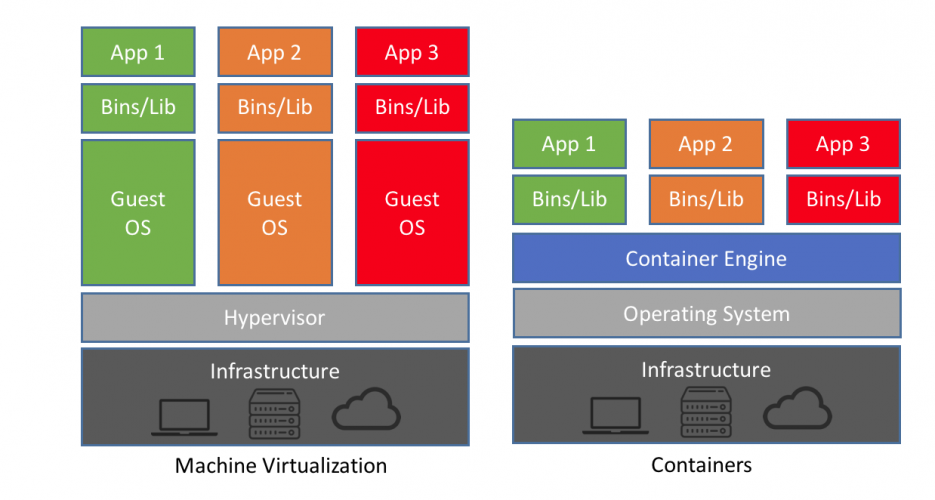
\includegraphics[width=0.9 \columnwidth]{Images/VM_vs_container.png}
\end{center}
\caption{Virtual machine vs container~\citep{Container-vs-vm}}
\label{fig:container_vs_vm}
\end{figure}

\newpage

Linux containers (LXCs) provide several features to manage applications running in them, the most important ones being control groups (cgroups) and namespaces. Cgroups provide a unified interface to manage processes and their resources, including resource monitoring and limiting, prioritization and control~\citep{Cgroup}. Namespaces are used to isolate a processes' resources. This makes it appear to the processes within the namespace that they have access to their own isolated instance of a global resource~\citep{Namespace}.

\subsubsection{Docker}
Docker is a container engine designed to manage Linux containers. It offers functionalities to develop, ship and run applications through container-based virtualization~\citep{Docker}. Containers in Docker are created through Docker images, which are read-only templates with instructions for creating the Docker container~\citep{Docker-image}. How to build a Docker image is, in turn, documented in a Dockerfile. Figure \ref{fig:dockerfile} shows an example Dockerfile. Docker is, however, limited to the management of containers on a single machine.

\begin{figure}
\begin{center}
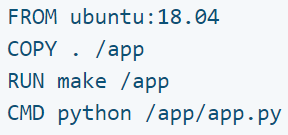
\includegraphics[width=0.35 \columnwidth]{Images/Dockerfile.PNG}
\end{center}
\captionsetup{justification=centering}
\caption{Dockerfile example. FROM creates the starting layer, COPY adds files, RUN executes a command and CMD provides the default command and arguments for the container~\citep{Dockerfile}.}
\label{fig:dockerfile}
\end{figure}

\subsection{Kubernetes}
When deploying applications in a distributed context, managing them becomes a challenge. Container orchestration engines like Kubernetes provide multiple features to manage distributed systems effectively. Kubernetes is an open source container orchestration engine providing basic mechanisms for the deployment, maintenance, and scaling of applications~\citep{kubernetes_github}.

\subsubsection{Terminology}

\paragraph{Pod} A pod is the smallest deployable unit in Kubernetes, as mentioned in the introduction. It encapsulates one or more containers, storage resources and a unique network IP. Each pod is meant to run a single instance of a given application. Figure \ref{fig:pod} shows an example definition of a pod definition~\citep{Kubernetes-Pod}.

\begin{figure}
\begin{center}
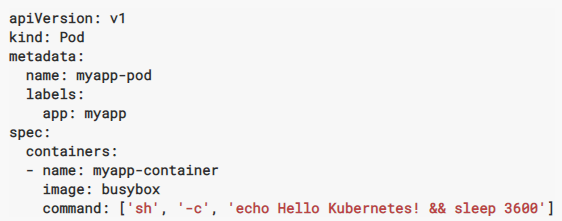
\includegraphics[width=0.90 \columnwidth]{Images/Pod_example.PNG}
\end{center}
\captionsetup{justification=centering}
\caption{Pod definition example. The pod contains one container, called \textit{`myapp-container'}, which is based on the \textit{`busybox'} Docker image~\citep{Kubernetes-Pod}.}
\label{fig:pod}
\end{figure}

\paragraph{ReplicaSet}
If multiple replicas of identical pods ar required to run at all times for, for example, availability purposes, a ReplicaSet can be defined. A ReplicaSet's definition includes the specifications of the pod and the amount of replicas which should be maintained~\citep{Kubernetes-ReplicaSet}.

\paragraph{Deployment}
Pods and ReplicaSets may need to be updated during operations. A Deployment describes the desired state of either a pod or a ReplicaSet. Typical use cases of Deployments are:
\begin{itemize}
    \item Rolling out a ReplicaSet by creating a Deployment;
    \item Declaring the new state of a pod by updating a Deployment;
    \item Rolling back to an earlier Deployment;
    \item Scaling up or down the amount of replicas;
    \item Pausing and resuming a Deployment to apply fixes;
    \item Checking the status of a Deployment; and
    \item Removing unused ReplicaSets~\citep{Kubernetes-Deployment}.
\end{itemize}

\paragraph{StatefulSet}
StatefulSets are similar to Deployments but provide additional guarantees about the ordering and uniqueness of the pods. They are typically used when any of the following features is desired:
\begin{itemize}
    \item Stable and unique network identifiers;
    \item Stable and persistent storage;
    \item Ordered and graceful deployment and scaling; and
    \item Ordered and automated rolling updates \cite{Kubernetes-StatefulSet}.
\end{itemize}

\paragraph{Service}
Pods, by themselves, terminate without healing if anything goes wrong. ReplicaSets maintain a stable amount of identical pods, but the pods may be killed and recreated at any time. Since each pod gets its own IP address, the IP adress at which an application can be reached is subject to change. Services solve this problem by defining a set of logical pods and a policy by which to access them. Other applications then communicate with the application by addressing its Service~\citep{Kubernetes-Service}.

\paragraph{Requests and limits}
Users may specify the requests and limits of a pod. A pod is always guaranteed to get its requested amount of resources, and may use up to its specified limit when there are free resources in the node. The sum of the requests of all the pods running in a node should be less than or equal to the total amount of available resources of that node. The sum of limits, however, can be higher than the available resources of the node, allowing for oversubscription of that node. At the time of writing, Kubernetes only supports requests and limits for CPU and memory~\citep{requestlimit}.

\paragraph{Quality of Service classes}
Based on the requests and limits of a pod, Kubernetes automatically assigns it a Quality of Service (QoS) class. A pod is assigned the `Guaranteed' QoS class if every container in the pod has specified limits and optionally requests, and if the requests are all equal to the limits. A pod is assigned the `Burstable' QoS class if requests and optionally limits are set for any container in the pod, and they are not equal. If no requests or limits are set for any container in the pod, the pod gets the `Best Effort' QoS class~\citep{QoS}.

\subsubsection{Kubernetes out-of-resource handling}\label{background:oversubscription}

In an oversubscribed node, Kubernetes divides the free resources among the pods based on their requests, limits and QoS classes. When the workload grows, pods may need to contend for the free resources in the node. Depending on the type of the bottleneck resource, one of two things can happen. If the resource is compressible (able to be throttled), CPU for example, then the pod with the lowest request gets throttled. This allows the pod with the higher request to use a bigger part of the free resources. If the bottleneck resource is not compressible, like memory, the pod with the lowest QoS class gets evicted instead. \\

Kubernetes throttles pods as follows. It converts the requested CPU to its core value (so 500 millicores = 0.5 CPU) and multiplies it by 1024. A pod's \textit{cpu-shares} value is then set to the greater of this calculated number or 2~\citep{Kubernetes-cpu-shares}. When there are sufficient CPU cycles available for all containers, each container may use as much of them as needed, up to their specified limits. When CPU becomes limited, however, it is divided according to the relative weight of the \textit{cpu-shares} values. So, for example, if two containers have CPU requests of respectively \textit{1000m} and \textit{500m}, then, when CPU becomes limited, the first container receives 66\% of the CPU cycles, while the second one only receives 33\%~\citep{Docker-cpu-shares}.\\

\subsection{Autoscaling}
The goal of an autoscaler is to automatically adjust an application's resources based on its needs at any given time. Three main characteristics distinguish autoscalers. 
The first one is when it decides to scale, also referred to as the scaling model. This can be either reactively or proactively. Reactive approaches, as the name suggests, react to changes without anticipating them, while proactive approaches use forecasting techniques to determine when an application should be scaled. Some autoscalers use a combination of proactive and reactive approaches. 
A second characteristic is how the actual scaling is performed, also known as the scaling method. This can be through vertical scaling, horizontal scaling or a combination of both. Vertical scaling entails increasing the capacity of existing entities in the system. For example, if an application is deployed using virtual machines, the amount of memory to which a virtual machine has access could be increased or decreased. Horizontal scaling is achieved by adding or removing entities to the system, for example by adding or removing virtual machines. The third characteristic is which metrics are considered when making scaling decisions, for example CPU or memory usage~\citep{CoutinhoEmanuel2015Eicc}. 

\subsubsection{Autoscaling in Kubernetes}
As mentioned before, Kubernetes offers a default horizontal autoscaler called the Horizontal Pod Autoscaler (HPA)~\citep{HPA}. It is a purely reactive autoscaler which only bases its scaling decisions on CPU utilization by default. The HPA can be extended to support other scaling metrics. It makes scaling decisions using threshold-based policies. With such policies, certain thresholds are set for resource utilization or SLA violations and when they are crossed, the application should be scaled. Care has to be taken when implementing these thresholds, as oscillating metrics could lead to unnecessary scalings. An example of an unsafe or incomplete rule set would be ``if memory usage is greater than 80\%, a replica should be added'' paired with ``if memory usage is less than 80\%, a replica should be removed''. When the memory usage oscillates around 80\%, the autoscaler may decide constantly change the amount of replicas. This is sometimes referred to as thrashing. A better rule would be ``if memory usage is greater than 80\% for 5 minutes, the a replica should be added'', and vice versa. The Kubernetes HPA offers such thrashing prevention by including a certain scaling delay by default.\\

The Kubernetes community is also working on a Vertical Pod Autoscaler (VPA)~\citep{VPA}. A drawback of this autoscaler is that it needs to restart a pod when scaling it. Moreover, this autoscaler is not included by default.



\section{Related work}
\label{chap:existing_research}
This section describes recent work relevant to this paper. %Section \ref{surveys} discusses three works which bundle studies related to autoscaler technologies. Sections \ref{caravel} and \ref{hyscale} discuss two recently developed autoscaling solutions. At the end of each section, a small reflection of the work and its relevance, is given.
%
%\subsection{Surveys}
%\label{surveys}
%Eddy: Maybe this paragraph is useful for the intro
%During the last few years, extensive research concerning autoscalers has been
%conducted, and it is still very much ongoing. Multiple surveys have been published which attempt to provide an overview of the existing autoscaler research. In 2014, Lorido-Botran et al.~\citep{Lorido-BotranTania2014ARoA} classified and described popular autoscaling techniques and carried out a survey of the literature on autoscaling systems.\newline
%A more elaborate survey has been conducted by Coutinho et al.~\citep{CoutinhoEmanuel2015Eicc} and was published in 2015. Besides classifying articles related to autoscaling by the model and method discussed, the survey makes additional classifications based on the type of cloud platform, main benchmarking tools, test traces and scaling metrics used.\newline
%In an even more recent study~\citep{Al-DhuraibiYahya2018EiCC}, published in 2017, Al-Dhuraibi et al. bundle and describe literature about state of the art autoscalers and list several open issues regarding the topic. When classifying autoscaler literature, the paper makes even more distinctions, a notable one being whether the literature handles hypervisor-based or container-based infrastructure.
%
%\subsubsection{Open issues and research challenges}
%The three papers discussed above each listed open issues and research challenges.
%The most relevant ones concern resource granularity, start-up time, container-based virtualization and hybrid solutions:

%\paragraph{Resource granularity} Coutinho et al. mention how most autoscaling solutions use virtual machines as a scaling unit and how this forces clients to acquire fixed amounts of resources only. The paper also states that ``it would be very interesting to see the development of solutions to allow a fine-grained allocation of resources through the use of vertical scaling techniques''. Al-Dhuraibi et al. also describe this challenge and comment that ``vertical elasticity is very important to provide a related combination of resources according to the demand''.~\citep{CoutinhoEmanuel2015Eicc}~\citep{Al-DhuraibiYahya2018EiCC}

%\paragraph{Start-up time} 
%Lorido-Botran et al. conclude that ``reactive autoscaling systems might not be able to cope with abrupt changes in the input workload''. Similarly, Coutinho et al. mention that purely reactive autoscaling solutions may be too slow, as a certain start-up time is required for new resources to activate. Al-Dhuraibi et al. also list start-up time as an open issue of autoscalers, emphasizing that ``the lower the start-up time is, the better the elastic solution is''.~\citep{Lorido-BotranTania2014ARoA}~\citep{CoutinhoEmanuel2015Eicc}~\citep{Al-DhuraibiYahya2018EiCC}

%\paragraph{Container-based virtualization}
%Coutinho et al. state that container-based elastic solutions could be promising ``since containers can reduce the start-up time of replicas, as well as they have a resource management component for limiting the use of resources and metrics for monitoring''. Al-Dhuraibi et al. state that using elasticity-solutions defined for traditional hypervisor-based solutions in a container-based environment is still an open challenge.~\citep{CoutinhoEmanuel2015Eicc}~\citep{Al-DhuraibiYahya2018EiCC}

%\paragraph{Hybrid solutions} Lorido-Botran et al. advise to ``take advantage of the prediction capabilities of time series analysis techniques, together with the automation capabilities of controllers''. Coutinho et al. identify several hybrid approaches to autoscaling and mention that ``combining reactive and proactive approaches seems to be a good idea''. Al-Dhuraibi et al. also mention that besides combining proactive and reactive approaches, combining vertical and horizontal scaling could prove useful.~\citep{Lorido-BotranTania2014ARoA}~\citep{CoutinhoEmanuel2015Eicc}~\citep{Al-DhuraibiYahya2018EiCC}

%\subsubsection{Discussion}
%This paper relates closely to the open issues mentioned above. It explores whether the oversubscription concepts described in section \ref{background:oversubscription} allow for fine-grained vertical scaling of Kubernetes pods. Furthermore, it evaluates whether the usage of the Kubernetes HPA in combination with these oversubscription mechanisms provides additional cost-efficiency benefits.
%
%\subsection{Caravel}
%\label{caravel}
Caravel~\citep{caravel} is a scheduler developed by Deshpande et al. which co-schedules stateful and stateless applications in containerized environments. Stateful applications require more care to schedule when compared to stateless applications, as each replica of a stateful application is unique and the order of scheduling matters. When scaling out, stateless applications can scale instantly by spawning an identical copy. Scaling stateful applications requires more planning and is thus also slower in most cases. This makes vertical scaling the preferred method of scaling for stateful applications during a load peak, as no new replicas need to be scheduled. Vertically scaling stateful applications entails its own risks, however. In container orchestration frameworks, applications using more than their requested amount of resources risk being evicted. In turn, a second problem called burst propagation arises: %Most container orchestration frameworks do not consider the type of application when evicting. The impact of evicting a specific container is also not considered. Evicting a stateful application leads to the application needing to be restarted. This is, as discussed earlier, a slow process which decreases the ability to handle sudden load peaks even more. Caravel addresses these concerns by allowing stateful applications to use more than their requested amount of resources during load peaks.
%
%\subsubsection{Evicting stateful containers}
%Evicting a stateful container is undesirable for several reasons, as described by Deshpande. The first one is that a stateful container's state can be lost when it is evicted. A Redis~\citep{redis} database cluster consisting of two replicas serves as an example. Updates to the database are executed in both replicas. When one replica gets evicted, it loses all its state since Redis is an in-memory database. When restarting, said state needs to be recovered by synchronizing with the other replica. This synchronization also leads to the other replica's resources being used, which in turn causes an even worse performance~\citep{caravel}. \\
%A second problem when evicting pods is called burst propagation.  When a load peak occurs, a container could scale vertically and use more resources than it requested. This could result in the container being evicted, as discussed. 
Eviction of one replica results in the load being redirected to another replica. Now this replica's resource usage increases and it will in turn be prone to eviction, and so on. Another option for container orchestration frameworks is to throttle the resources of a container instead of evicting it, but this will cause a drop in performance during load peaks~\citep{caravel}.
%Deshpande illustrates that horizontally scaling a stateless application (Nginx) only takes a few seconds, while scaling Redis, a stateful application, takes approximately 5 minutes. Still, eviction of stateful applications cannot be avoided completely, especially in an environment where a large fraction of the applications are stateful. In that case, a scheduler needs mechanisms to ensure fairness in eviction. Eviction can also be unavoidable when containers fail, are upgraded or are moved to other nodes. Furthermore, a scheduler needs to take into account past evictions when scheduling future ones~\citep{caravel}.\\

Deshpande et al. developed an eviction algorithm that addresses these concerns by letting stateful containers evict stateless containers as these can be restarted in only a few seconds on another node. However, each stateful application can only evict a limited number of containers, limiting the effects of large bursts. The total amount of resources acquired simultaneously by all stateful applications is also limited to prevent them from overwhelming the cluster. Finally, future evictions are spread fairly across applications. 
This approach thus tolerates bursty behavior of stateful applications and reduces their evictions by preferring to evict stateless containers. It also imposes a mechanism to control excessive evictions of stateless applications. This paper explores how similar behavior could be achieved by only using Kubernetes mechanisms. However, the distinction is not made between stateful and stateless applications but rather between high and low priority applications. 

Wong et al.~\citep{hyscale} describes the (dis)advantages of vertical and horizontal scaling and proposes a hybrid solution. 
%The hybrid solution aims to reap the benefits of the fine grained resource control and the high availability of vertical and horizontal scaling respectively. 
%
%\subsubsection{Hybrid scaling difficulties}
%Designing a hybrid scaling algorithm comes with several challenges, as explained by Wong. The problem of finding an optimal configuration starts from numerous parameters: CPU, memory usage, network usage, a limited number of physical resources and a set of microservices with variable dimensions. These parameters may be tied to one another. Finding a solution to this problem is NP-complete, but in practice, it must be determined in real-time. A second problem is that the optimal configuration may fluctuate, especially when the user load is unstable or bursty. This can lead to excessive overhead due to thrashing.\\
%
%\subsubsection{Horizontal versus vertical scaling}
%Wong performs a series of small experiments to study which scaling method is preferable for which contended resource. 
The solution is developed on top of Docker engine without any container orchestration framework. 
%For CPU resources, their results show a preference for vertical scaling as it provided negligible overhead. With horizontally scaling, on the other hand, CPU performance decreases as the amount of replicas increases, as shown in Figure \ref{fig:hyscale1}. This performance decrease becomes even larger when replicas are located on different nodes. When memory is the contended resource, Wong shows that the difference between the two scaling methods is negligible and that most overhead is application specific~\citep{hyscale}.\\
%
%\begin{figure}
%\begin{center}
%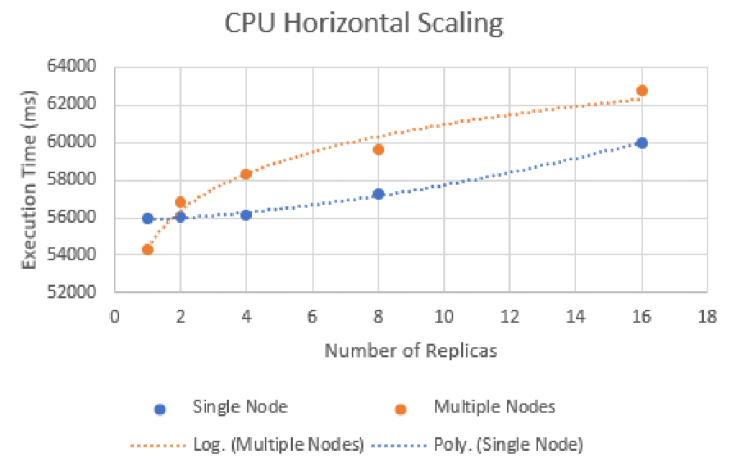
\includegraphics[width=0.65\columnwidth]{Images/Related_work/Hyscale_1.PNG}
%\end{center}
%\caption{Horizontal scaling response times for CPU tests~\citep{hyscale}}
%\label{fig:hyscale1}
%\end{figure}
%
Wong compares their scaling solution to the standard autoscalers in Kubernetes. A first disadvantage noted by Wong is that the default Kubernetes scaling solutions only consider one resource when making scaling decisions. Second, Wong explains how the Kubernetes autoscalers often lead to sub-optimal configurations. 
The HyScale algorithm differs from the default Kubernetes HPA in two ways: the use of vertical scaling and the consideration of multiple metrics to make scale decisions. 
A complete discussion of the algorithm does not fall within the scope of this paper. 
Wong's experimental results show that HyScale outperforms Kubernetes for bursty workloads. For non-bursty workloads, their performance is similar
~\citep{hyscale}.

When comparing horizontal and vertical scaling for CPU intensive workloads, Wong describes that Docker's CPU shares mechanism can be used to ``induce a form of vertical scaling, as increasing or decreasing shares directly correlate with an increase or decrease in CPU resource allocation to a container''~\citep{hyscale}. When comparing the HyScale solution to Kubernetes, however, they only consider the Kubernetes HPA, without mentioning these CPU shares. This paper evaluates the effects of combining the HPA with the CPU shares mechanism in Kubernetes. 


%\setlength\abovecaptionskip{0pt}
\section{Test Environment}
\label{chap:test_env}


This section describes the specific tools used in the experiments and a brief overview of the three test applications. 

%This section describes the specific tools used in the experiments. It starts with presenting the deployed Kubernetes cluster's layout. Then, the tools needed to run the actual experiments are introduced. Finally, this section concludes with a brief overview of the three test applications used.

\paragraph{Kubernetes cluster.}
\label{cluster}
All the experiments are run on a Kubernetes cluster deployed on the DistriNet private cloud, which is based on the OpenStask platform~\citep{openstack}. Four virtual machines are deployed: one master and three worker nodes. The cluster itself is created using \textit{kubeadm}~\citep{kubeadm}. All of the machines are running the Ubuntu 16.04 operating system. Three of the nodes, including the master node, are allocated 2 CPUs and 4 GB of memory. The last node is assigned 4 CPUs and 8 GB of memory. The three worker nodes are placed on the same OpenStack computing node to minimize latencies between applications running on the nodes. On the first worker node, which is the node with 4 CPUs and 8GB of memory, an experiment controller is deployed. The second and third worker nodes are reserved for the applications to be deployed on. An overview of the setup is shown in Figure \ref{fig:cluster}.

\begin{figure}
\centering
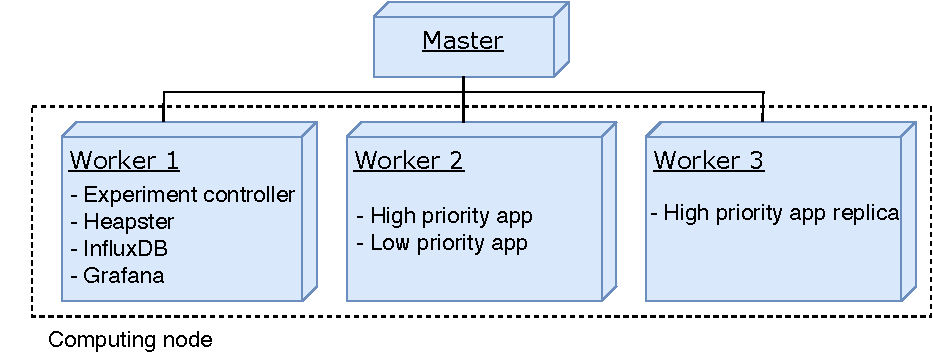
\includegraphics[width=0.80\columnwidth]{Images/Setup/Cluster.pdf}
\caption{Test cluster setup}
\label{fig:cluster} 
\end{figure}


\paragraph{Experimentation tools.}
\label{tools}
%
%\subsubsection{Resource monitoring}
To monitor the resources in the cluster, a combination of Heapster~\citep{heapster}, InfluxDB~\citep{influxdb} and Grafana~\citep{grafana} is employed. To run and monitor the experiments, K8-Scalar~\citep{scalar} is used. K8-Scalar is an extensible workbench exemplar for implementing and evaluating different self-adaptive approaches to autoscaling container-orchestrated services~\citep{scalar-github-overview}.
%Heapster collects each node's metrics through the kubelet node agent~\citep{kubelet}~\citep{heapster-influxdb-grafana}. The collected data is written to InfluxDB. InfluxDB is a time-series database, a database optimized for time-stamped or time series data~\citep{timeseriesdb}. Grafana is a metric dashboard and graph editor which supports, among others, InfluxDB~\citep{grafana-github}. 

%\subsubsection{Experiment controller}
 
%K8-Scalar can be customized to test a specific system by implementing Java user and request classes fit for that system. Multiple users may be implemented, for example one user which performs CPU-intensive requests and one which performs memory-intensive requests. When preparing an experiment, the distribution of the types of users can be specified, for example 95\% of the users executing memory intensive requests and 5\% executing CPU intensive requests. Furthermore, the exact workload profile can be described using a template.
%, part of which is shown in listing \ref{listing:profile}
%An experiment in K8-Scalar consists of multiple runs, and the peak load for each of these runs must be provided. A run in turn consists of a ramp-up phase, a peak load phase and a ramp-down phase. The duration of all of these phases can be configured. In between runs, there can also be constant low load phases. Ramping up and down is done linearly. Besides sending the requests, K8-Scalar monitors the time needed by the tested applications to process these requests~\citep{scalar}.
%
%\lstset{caption={Load profile example},label=listing:profile}
%\begin{lstlisting}[float]
%## LOAD PROFILE
%user_peak_load=500,1000,1500
%user_warmup_fraction=1
%user_warmup_duration=0
%user_ramp_up_duration=0
%user_peak_duration=400
%user_ramp_down_duration=0
%user_cooldown_duration=0
%user_wait_inbetween_runs=0
%\end{lstlisting}
%
\subsection{Deployed applications}
\label{test-apps}

\paragraph{Cassandra based application.}
A Cassandra based application is selected as the first high priority test application. Only write operations are examined in this paper, as they are CPU intensive. The main QoS requirement for the application is thus the latency of write requests. Cassandra is well-suited for the experiments as its design is optimized for write-heavy workloads~\citep{scalar}.

\paragraph{Artificial SaaS application.}
\label{setup:saas-app}
An artificial SaaS application developed at KU Leuven~\citep{saas-app} is selected as a second high priority test application. The main benefit of this SaaS application is that the stressed resource is easily configurable through the application's REST interface. For example, if a CPU intensive workload needs to be tested, the memory intensity of the application can be set to zero by executing a simple REST command at runtime. 

\paragraph{Low priority application.}
\label{setup:lpp}
%The application shown in Figure \ref{fig:cpu-app-python} is deployed as t
The low priority application used for testing the effects of co-locating pods executes a multiplication in an infinite loop. If sufficient resources are free, it continually uses a full CPU since it is single threaded. The exact CPU usage is known and roughly constant.

%\setlength\abovecaptionskip{-5pt}

\section{Results}
\label{chap:results}
In this section, the Kubernetes mechanisms for resource management are evaluated through a series of experiments. 

\subsection{Experiment 1: Determining the effects of request and limit configurations}
If there is just one pod scheduled on a node, and if that pod has no limits set, then it should be able to use all of the nodes resources. This experiment tests this hypothesis using a Cassandra application.

\paragraph{Setup.}
First, the expected performance of the Cassandra application is described in an SLO as follows:

\begin{slo}
95\% of the requests sent to the Cassandra application must be handled within 150ms, as measured by the experiment controller.
\end{slo}

The Cassandra application is deployed on the second worker node with a CPU and memory request of respectively \textit{1500m} and \textit{2GiB}. No limits are set. In this experiment, the experiment controller sends an increasing amount of requests to the Cassandra application, starting at 100 requests per second up to 600 requests per second, increasing with 50 requests every 600 seconds. 

\paragraph{Results.}
Figure \ref{fig:lat-cas-li} shows the 95th percentile latencies of the requests, as reported by the experiment controller. At around 400 requests per second, the SLO is violated. Figure \ref{fig:cpu-cas-li} shows the CPU usage of Cassandra and the second worker node. It illustrates that at around the same amount of requests per second, the node uses all of its available CPU, as 2.0K millicores equals 2 CPUs. This validates that the bottleneck is indeed the CPU. Furthermore, Figure \ref{fig:cpu-cas-li} shows that the Cassandra application is able to use almost all of the overprovisioned resources. This in in line with expectations, as the resources on the node are only contended by the Cassandra application.

\begin{figure}
\centering
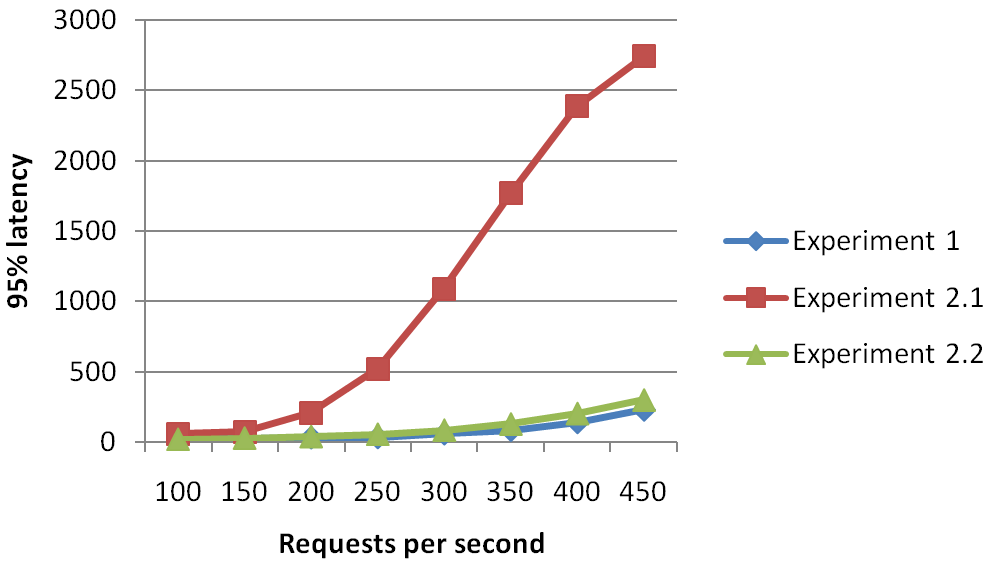
\includegraphics[width=0.75\columnwidth]{Images/Experiments/CPU/Latencies/lat-exp1-2.PNG}
\caption{95th percentile latencies during Experiment 1 and 2.}
\label{fig:lat-cas-li} 
\end{figure}

\begin{figure}
\centering
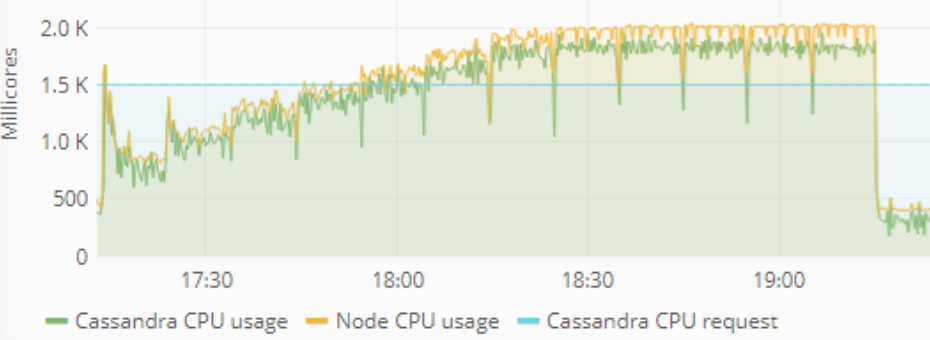
\includegraphics[width=0.80\columnwidth]{Images/Experiments/CPU/Grafana/cpu-cas-li.PNG}
\caption{Second worker node CPU usage during Experiment 1. The CPU usage of Cassandra rises above its CPU request, illustrating that the application can use all of the overprovisioned resources.}
\label{fig:cpu-cas-li} 
\end{figure}

%It should be verified that the experiment controller has sufficient resources to run the experiments. Preliminary tests show that the experiment-controller is CPU bound. Figure \ref{fig:cpu-scalar} shows the experiment controller's CPU usage during the experiment described above. A peak in CPU usage can be examined at the start of each run, but these peaks stay well below the available amount of CPU in the node. The experiment controller should thus not be the bottleneck during the experiments.
%
%\begin{figure}
%\centering
%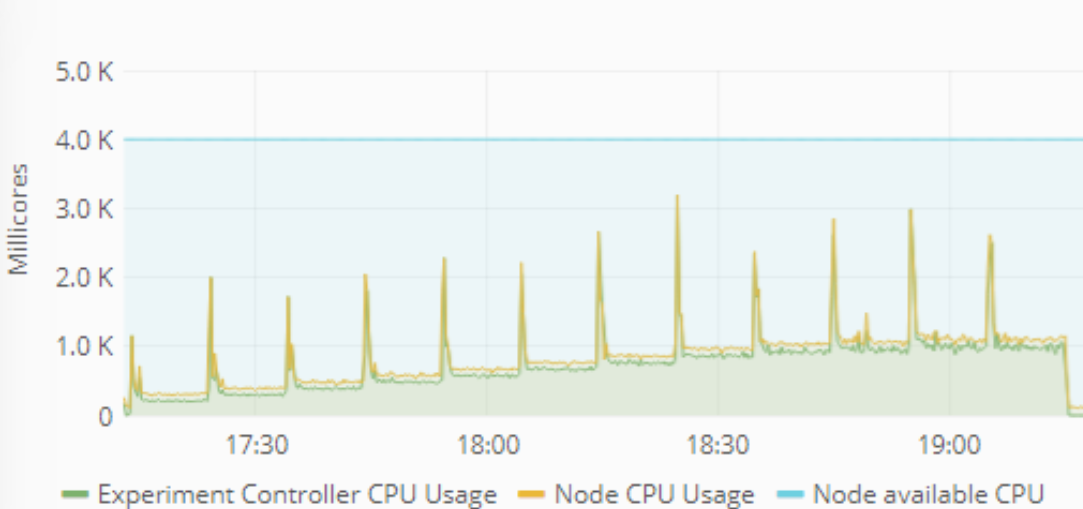
\includegraphics[width=0.80\columnwidth]{Images/Experiments/CPU/Grafana/cpu-scalar.PNG}
%\caption{Experiment controller CPU usage during Experiment 1. The node's CPU usage never reaches its capacity.}
%\label{fig:cpu-scalar} 
%\end{figure}

\subsection{Experiment 2: Determining the effects of co-locating a high and low priority application}
The goal of this experiment is to answer whether it is possible to increase cost-efficiency by using the Kubernetes oversubscription mechanisms described in \S1. Through two tests, we illustrate the effects of different request configurations when a high and low priority pod are co-located on a node.

\paragraph{Setup.}
The low priority application described in \S\ref{setup:lpp} is added to the second worker node as a low priority pod. The experiment consists of two separate tests. During the first one, Cassandra and the low priority pod each have a CPU request of \textit{500m}. For the second test, Cassandra has a CPU request of \textit{1500m} while the low priority pod has a CPU request of only \textit{10m}. The workload applied is the same as the one applied during Experiment 1. During the first test, both pods should receive an equal amount of CPU cycles. The results of the the test should indicate significantly higher 95th percentile latencies when compared to the results from Experiment 1, because the Cassandra pod cannot use all of the resources on the node. During the second test, Cassandra's performance should only be affected slightly due to the aforementioned \textit{cpu-shares} mechanism.

\paragraph{Results.}
Figure \ref{fig:cpu-cas-lpp-li} shows the CPU usage of both the Cassandra pod and the low priority pod during the first test, when their requests are equal. It shows that the available CPU is split equally between both pods. As expected, Figure \ref{fig:lat-cas-li} illustrates that the proposed  SLO gets violated at about half the amount of requests per second when compared to Experiment 1.

\begin{figure}
\centering
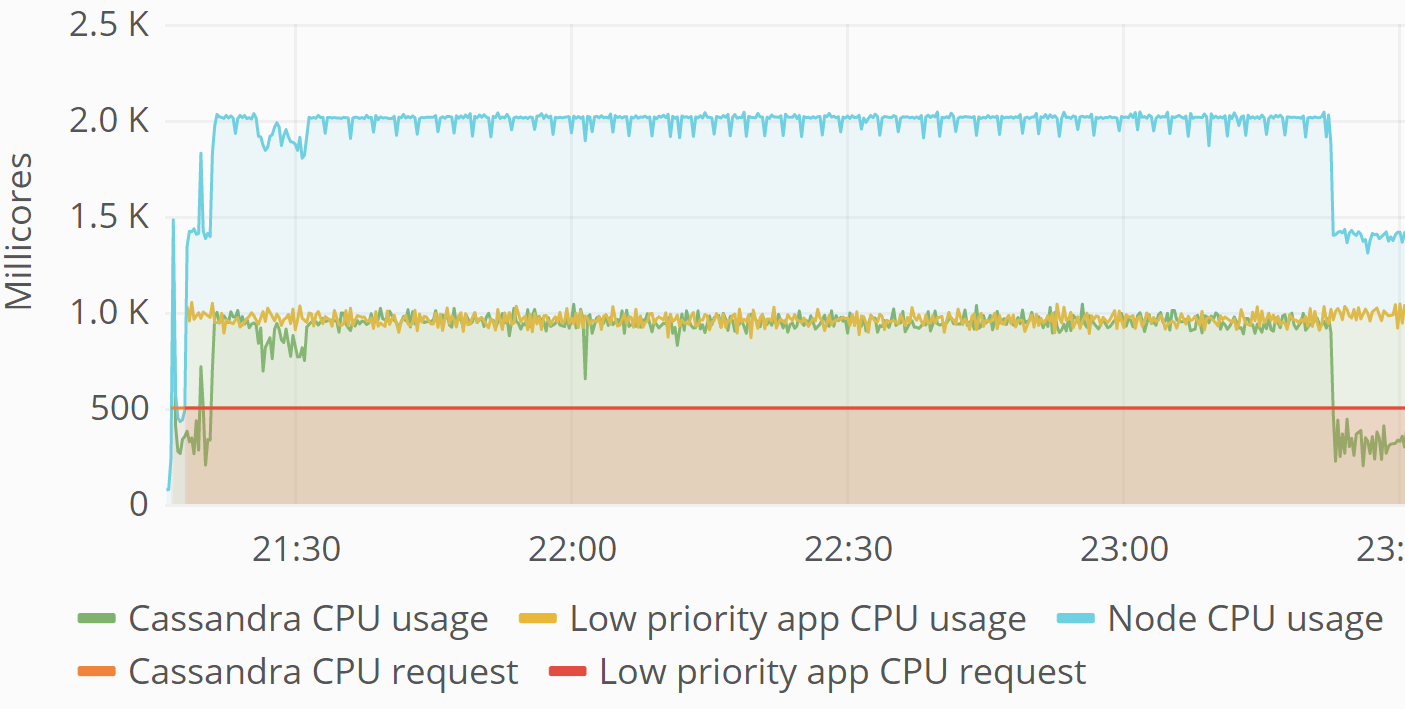
\includegraphics[width=0.90\columnwidth]{Images/Experiments/CPU/Grafana/cpu-cas-lpp-li.PNG}
\caption{Second worker node CPU usage during the first test of Experiment 2. The deployed applications receive an equal share of the available CPU.}
\label{fig:cpu-cas-lpp-li}
\end{figure}

%\begin{figure}
%\centering
%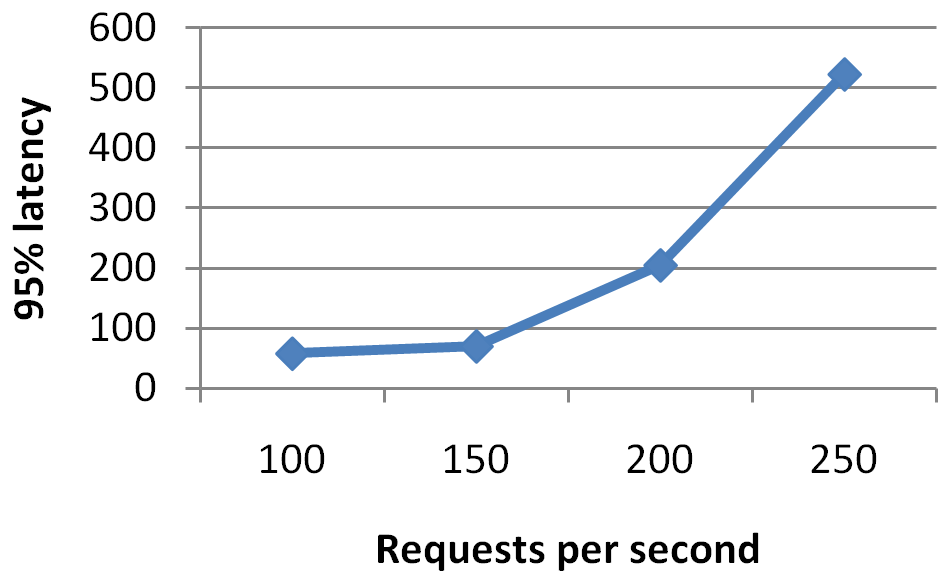
\includegraphics[width=0.50\columnwidth]{Images/Experiments/CPU/Latencies/lat-cas-lpp-li.PNG}
%\caption{95th percentile latencies during the first test of Experiment 2. The proposed SLO is violated at around 200 requests per second. Compared to Experiment 1, %the Cassandra application is able to process only half the amount of requests per second as a result of it only having access to half of the resources.}%
%\label{fig:lat-cas-lpp-li}
%\end{figure}
%
Figure \ref{fig:cpu-cas-lpp-li-2} shows the worker node's CPU usage during the second test of this experiment. As the amount of CPU needed by the Cassandra pod increases, the amount of CPU available to the low priority pod decreases, which is according to expectations. The 95th percentile latencies shown in Figure \ref{fig:lat-cas-li} illustrate a slight increase of latencies when compared to the Experiment 1.

%\begin{figure}
%\centering
%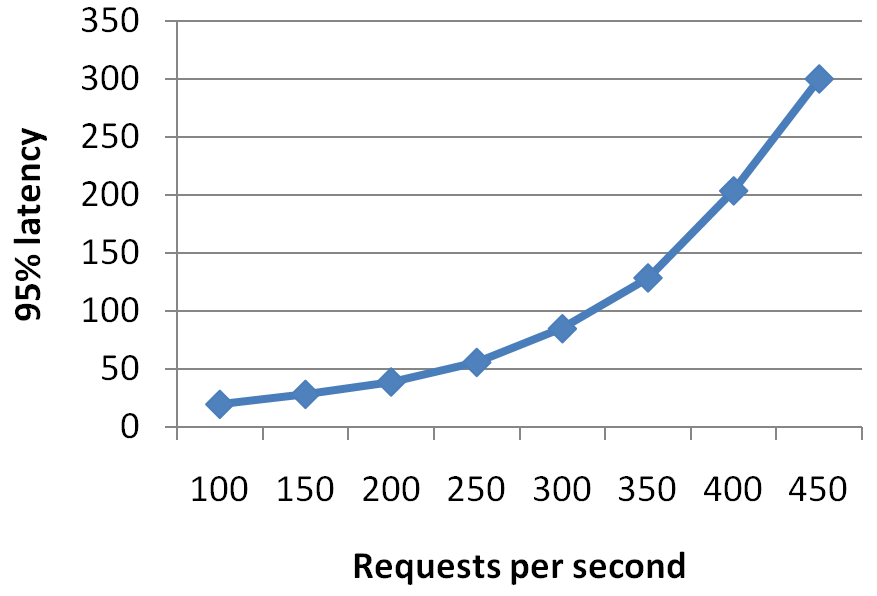
\includegraphics[width=0.50\columnwidth]{Images/Experiments/CPU/Latencies/lat-cas-lpp-li-2.PNG}
%\caption{95th percentile latencies during the second test of Experiment 2. The latencies are comparable to the ones examined during Experiment 1, showing that %performance is only slightly impacted.}
%\label{fig:lat-cas-lpp-li-2}
%\end{figure}

The slight decrease in performance comes with the benefit of a higher resource utilization. Comparing the worker node's total CPU usage during Experiment 1 to the node's total CPU usage in this test, the latter shows a significantly higher resource utilization when the workload of the Cassandra pod is low.

\begin{figure}
\centering
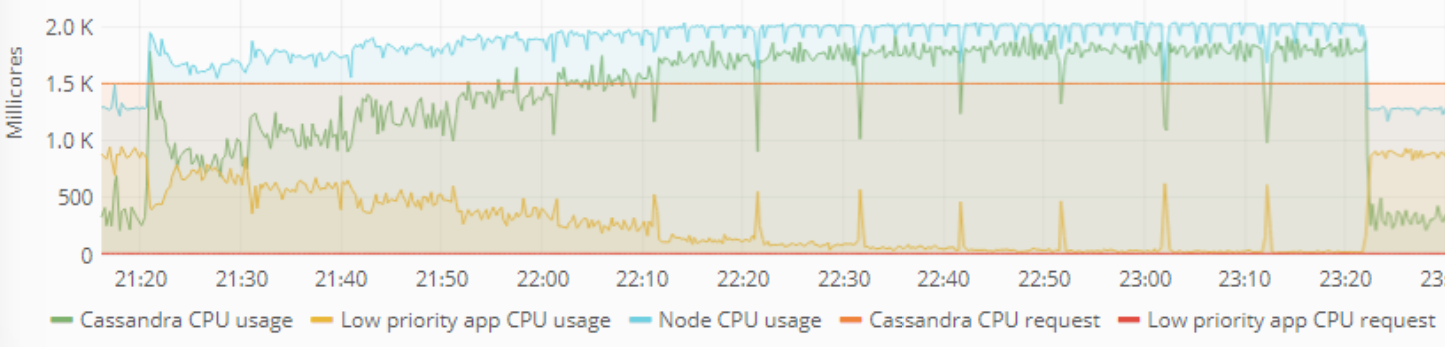
\includegraphics[width=\columnwidth]{Images/Experiments/CPU/Grafana/cpu-cas-lpp-li-2.PNG}
\caption{Second worker node CPU usage during the second test of Experiment 2. As the Cassandra workload rises, the amount of CPU cycles granted to the low priority application decreases.}
\label{fig:cpu-cas-lpp-li-2}
\end{figure}

\subsection{Experiment 3: Determining the effects of bursty workloads}
In this experiment, a bursty workload is applied to examine its effects on Cassandra's performance. In the previous experiment, Cassandra could process 350 requests per second without violating the proposed SLO. This experiment should clarify whether Kubernetes can divide resources in time so that Cassandra can process the bursts of 350 requests per second without violating the SLO.

\paragraph{Setup.}
The setup for this experiment is equal to the one used in Experiment 2. In this experiment, 5 minutes of a manageable workload (200 requests per second) is applied, followed by a one minute burst of 350 requests per second. This pattern is repeated 20 times.  

\paragraph{Results.}
Figure \ref{fig:cpu-cas-lpp-bursty} shows the resource utilization during this experiment. It depicts the expected behavior: during a burst, CPU cycles are taken away from the low priority application and granted to the high priority one. The low priority application is allowed to use more resources in between bursts, increasing cost-efficiency. The experiment controller reported an average 95th percentile latency of \textit{109.3 ms} during the bursts, which is comparable to the latencies reported during the previous experiment at 350 requests per second. The type of workload, bursty or more seasonal, thus seems to have no effect on the operation of the \textit{cpu-shares} mechanism. 

\begin{figure}
\centering
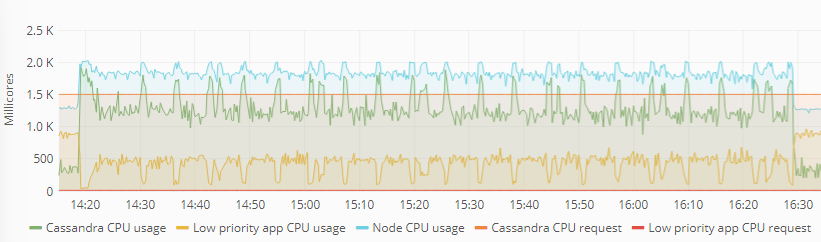
\includegraphics[width=\columnwidth]{Images/Experiments/CPU/Grafana/cpu-cas-lpp-bursty.PNG}
\caption{Second worker node CPU usage during Experiment 3.}
\label{fig:cpu-cas-lpp-bursty}
\end{figure}

\subsection{Experiment 4: Determining the effects of the Kubernetes HPA on Cassandra performance}
\label{exp:hpa-cass}
The goal of this experiment is to validate the correct performance of the HPA in combination with the application at hand, Cassandra. 

\paragraph{Setup.}
In this experiment, the HPA is added to the cluster, and the third worker node is made available to deploy a replica of the Cassandra application on. The low priority pod is removed from the cluster. The workload described in Experiment 1 will be applied to Cassandra. The HPA is configured to scale Cassandra when its CPU usage rises above 110\% of its CPU request, so at around \textit{1650 millicores}. 110\% is selected as the point to scale as spinning up a new replica takes some time. Scaling when the node's resources are fully used may be too late and may thus result in SLA violations. %The experiment controller divides the workload among all active replicas by sending the requests to the Cassandra application service, which takes care of the load balancing. 

\paragraph{Results.}
Figure \ref{fig:cpu-cas-hpa-li} shows the CPU usage of both the primary Cassandra pod and the replica added by the HPA. The graphs illustrate that a new Cassandra replica is added when scaling threshold is breached. Despite this, the load on the original Cassandra replica does not decrease when the new replica is activated. Since the experiment controller sends the workload to the Cassandra service, and this service should load balance over all available replicas, this is not in line with expectations. The 95th percentile latencies of the requests, shown in Figure \ref{fig:lat-cas-hpa-li}, reflect this unexpected behavior. Instead of the latencies going down when a new replica is added, they go up significantly.
%This can partially be explained by the fact that there is a certain warm-up associated with new Cassandra replicas: the first requests sent to a new Cassandra replica have higher latencies. This short-lived warm-up period explains the peak in latencies around 400 requests per second (the point of scaling), but does not justify the whole picture. 
The full explanation is beyond the scope of this paper. Truyen et al.~\citep{TruyenEddy2019Pooc} found that Kubernetes introduces a performance overhead when running Cassandra. %Additional experiments performed during this paper illustrated that this performance overhead increases significantly when more replicas are added. Scaling Cassandra in a native deployment, without using Kubernetes, did not cause major performance losses. In conclusion, the overhead was shown not to be caused by the HPA algorithm, but by Kubernetes itself.

\begin{figure}
\centering
\begin{subfigure}[b]{\columnwidth}
\centering
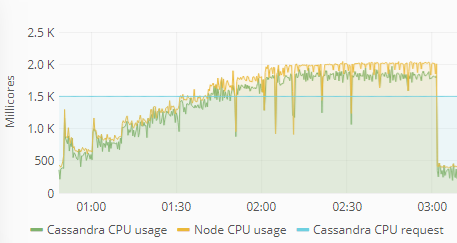
\includegraphics[width=0.70\columnwidth]{Images/Experiments/CPU/Grafana/cpu-cas-hpa-li-1.PNG}
\caption{Second worker node's CPU usage}
\label{fig:cpu-cas-hpa-li-1}
\end{subfigure}
\hfill
\begin{subfigure}[b]{\columnwidth}
\centering
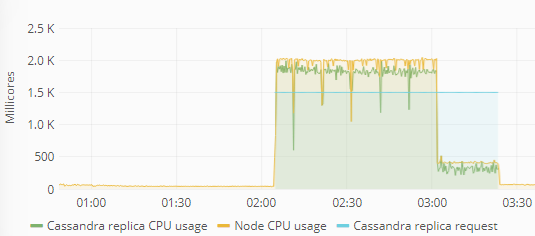
\includegraphics[width=0.70\columnwidth]{Images/Experiments/CPU/Grafana/cpu-cas-hpa-li-2.PNG}
\caption{Third worker node CPU usage}
\label{fig:cpu-cas-hpa-li-2}
\end{subfigure}
\hfill
\vspace*{-7mm}
\caption{CPU usage during Experiment 4. At 110\% of the CPU request, the given CPU threshold, a new Cassandra replica is added by the HPA. The CPU usage of the original replica does not decrease when the new replica is added, indicating scalability issues of Cassandra in Kubernetes.}
\label{fig:cpu-cas-hpa-li}
\end{figure}

\begin{figure}
\centering
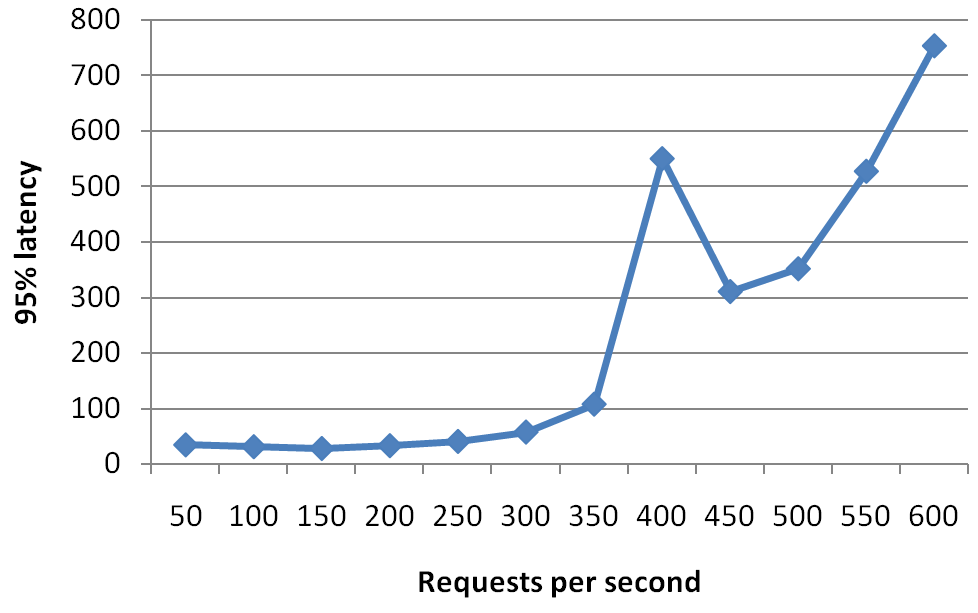
\includegraphics[width=0.55\columnwidth]{Images/Experiments/CPU/Latencies/lat-cas-hpa-li.PNG}
\caption{95th percentile latencies during Experiment 4. The latencies increase rather than decrease when a replica is added.}
\label{fig:lat-cas-hpa-li}
\end{figure}

\subsection{Experiment 5: Determining the effects of the Kubernetes HPA on the SaaS application performance}
The previous experiment is redone with the artificial SaaS application (introduced in \S\ref{setup:saas-app}) replacing Cassandra. Through two tests, this experiment verifies whether the performance of the SaaS application increases after a replica is added, or if it encounters the same scalability issues in Kubernetes as Cassandra.  

\paragraph{Setup.}
The SLO posed for the SaaS application is equal to the one posed for the Cassandra application in Experiment 1. Two separate tests are run. The first one subjects the SaaS application to a linearly increasing workload to see how much requests one replica can handle. The SaaS application's CPU request is set to 1.5 CPU and it is subjected to a linearly increasing workload similar to the one described earlier. For the second test, the HPA is added to the cluster and linearly increasing workload is again applied to the SaaS application. Again, 110\% of the request is selected as the point of scaling for the HPA. 


\paragraph{Results.}
Figure \ref{fig:lat-saas-li} shows the 95th percentile of latencies during this experiment. The SaaS application is able to process 150 requests per second without the HPA. Figure \ref{fig:cpu-saas-li} illustrates that at around 150 requests per second, the CPU in the node is fully used up, confirming that CPU is the bottleneck. With the HPA added, the application is able to process 250 requests per second without violating the SLO. This slightly less than double the 150 requests per second which the SaaS application can process without the HPA. Hence, there is still some overhead associated with having multiple replicas of the SaaS application, but it is relatively small compared to the overhead detected when scaling Cassandra in Kubernetes. Figure \ref{fig:cpu-cas-hpa-li-2} confirms that the workload is distributed over the replicas.

\begin{figure}
\centering
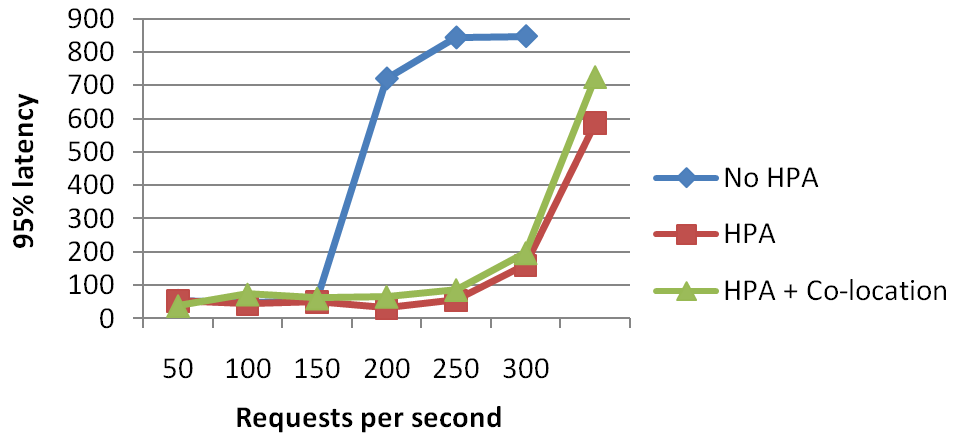
\includegraphics[width=0.75\columnwidth]{Images/Experiments/CPU/Latencies/lat-exp5-7.PNG}
\caption{95th percentile latencies during Experiments 5 and 7.}
\label{fig:lat-saas-li}
\end{figure}

\begin{figure}
\centering
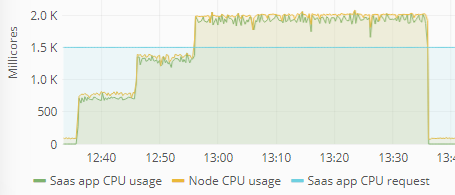
\includegraphics[width=0.70\columnwidth]{Images/Experiments/CPU/Grafana/cpu-saas-li.PNG}
\caption{Second worker node CPU usage during the first test of Experiment 5.}
\label{fig:cpu-saas-li}
\end{figure}

%
%\begin{figure}
%\centering
%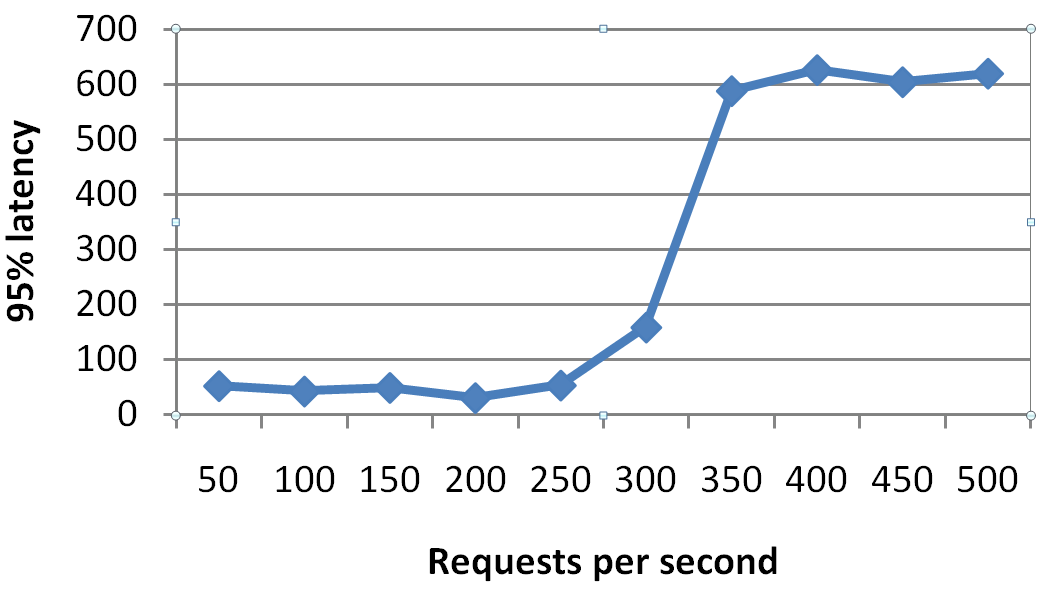
\includegraphics[width=0.60\columnwidth]{Images/Experiments/CPU/Latencies/lat-saas-hpa-li.PNG}
%\caption{95th percentile latencies during the second test of Experiment 5. The SaaS application can process a significantly higher amount of requests per second if an extra replica is added.}
%\label{fig:lat-saas-hpa-li}
%\end{figure}


\begin{figure}
\centering
\begin{subfigure}[b]{\columnwidth}
\centering
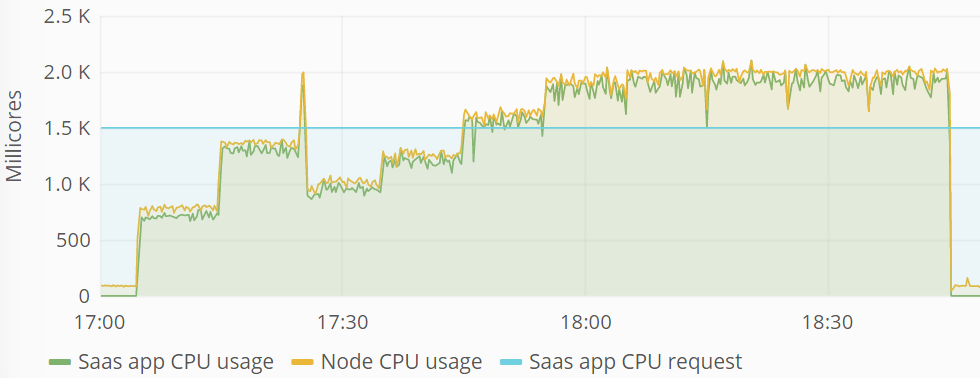
\includegraphics[width=0.70\columnwidth]{Images/Experiments/CPU/Grafana/cpu-saas-hpa-li-1.PNG}
\caption{Second worker node CPU usage.}
\label{fig:cpu-saas-hpa-li-1}
\end{subfigure}
\hfill
\begin{subfigure}[b]{\columnwidth}
\centering
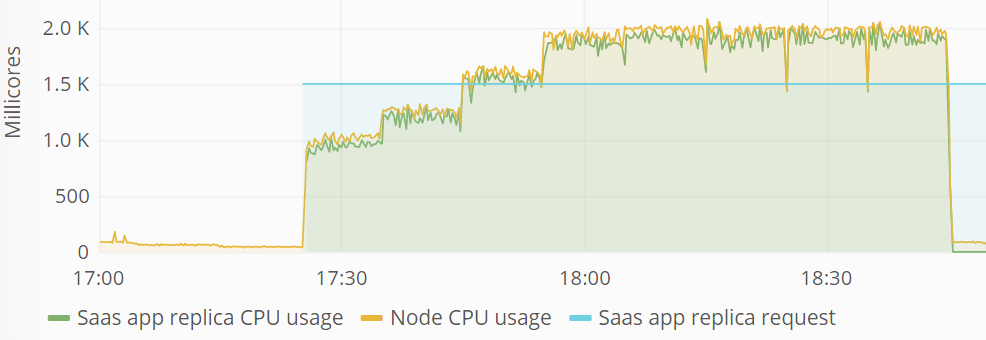
\includegraphics[width=0.75\columnwidth]{Images/Experiments/CPU/Grafana/cpu-saas-hpa-li-2.PNG}
\caption{Third worker node CPU usage.}
\label{fig:cpu-saas-hpa-li-2}
\end{subfigure}
\hfill
\vspace*{-7mm}
\caption{CPU usage during the second test of Experiment 5. The CPU usage of the original replica decreases when the HPA schedules a new replica of the SaaS application, confirming that the load is distributed among all replicas.}
\label{fig:cpu-cas-hpa-li-2}
\end{figure}

\subsection{Experiment 6: Determining the effects of bursty workloads on the performance of the Kubernetes HPA}
The goal of this experiment is to test how the Kubernetes HPA performs when the workload is bursty rather than linearly increasing. Even with the HPA added to the cluster, the SaaS application might not be able to process bursts of 250 requests per second, since starting a new replica can be slow. %The burst could be over by the time that the replica is fully started up.


\paragraph{Setup.}
The setup for this experiment is the same as the one used during the second test of the previous experiment. The bursty workload applied consists of five minutes of 60 requests per second followed by a one minute peak of 250 requests per second. This pattern is repeated 20 times.  

\paragraph{Results.}
Figure \ref{fig:cpu-saas-hpa-bursty} shows the worker node's CPU usages. The graphs illustrate that during the first couple of bursts, no scaling happens. This is unexpected since the scaling threshold is clearly breached. The 95th percentile latencies also report SLA violations during these bursts. One possible explanation is that the HPA does not poll the resource usage during the burst and thus does not notice the burst. This is, however, not the case, since the HPA queries the resource utilization every 15 seconds by default, and a burst lasts for 60 seconds. Another observation made from this experiment's results is that the HPA does not scale the application down after each burst. The HPA's algorithm details~\citep{hpa-algorithm-details} proved insufficient to find the cause of these inconsistent scaling decisions. 


\begin{figure}
\centering
\begin{subfigure}[b]{\columnwidth}
\centering
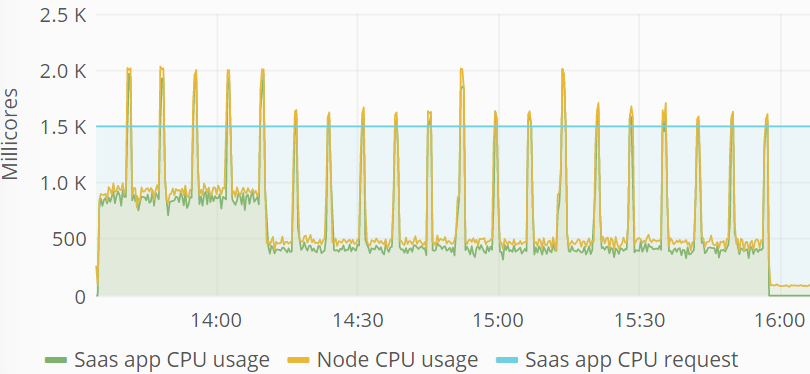
\includegraphics[width=0.75\columnwidth]{Images/Experiments/CPU/Grafana/cpu-saas-hpa-bursty-2-1.PNG}
\caption{Second worker node CPU usage.}
\label{fig:cpu-saas-hpa-bursty-2-1}
\end{subfigure}
\hfill
\begin{subfigure}[b]{\columnwidth}
\centering
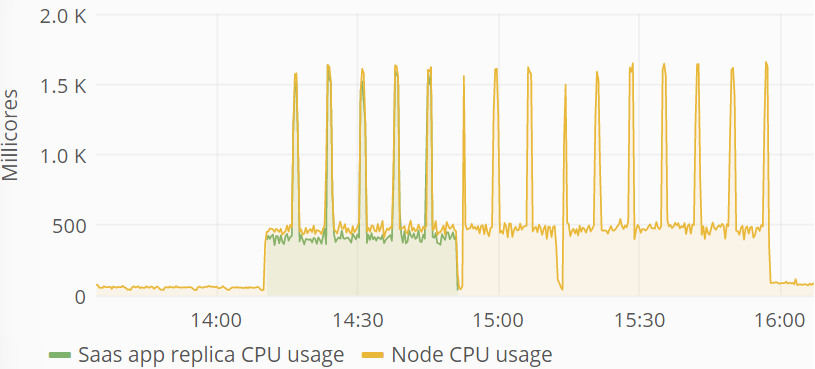
\includegraphics[width=0.75\columnwidth]{Images/Experiments/CPU/Grafana/cpu-saas-hpa-bursty-2-2.PNG}
\caption{Third worker node CPU usage.}
\label{fig:cpu-saas-hpa-bursty-2-2}
\end{subfigure}
\hfill
\vspace*{-7mm}
\caption{CPU usage during the first test of Experiment 6. Replicas are added and removed inconsistently.}
\label{fig:cpu-saas-hpa-bursty}
\end{figure}


It is possible that the HPA does not scale down the SaaS application since the default \textit{downscale stabilization} parameter of the HPA algorithm being five minutes~\citep{hpa-cooldown-delay}. This parameter specifies a period of time during which the HPA considers all recommendations before scaling down. In other words, the HPA only scales down if its decision to scale down has not changed for five minutes.
To verify this, another test is run where the downtime between each burst is set to 7 minutes. The other experiment parameters remain unchanged. Figure \ref{fig:cpu-saas-hpa-bursty-2} shows the CPU usage of the two worker nodes. During this test, the HPA scaled up the SaaS application during the first burst, but did not scale it down until after the test was completed. 

\begin{figure}
\centering
\begin{subfigure}[b]{\columnwidth}
\centering
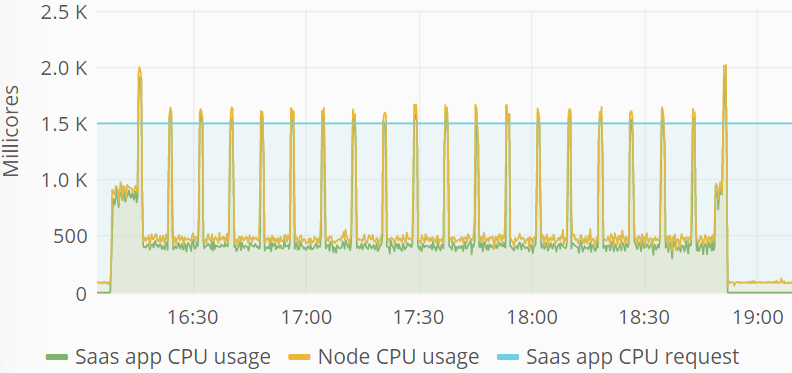
\includegraphics[width=0.70\columnwidth]{Images/Experiments/CPU/Grafana/cpu-saas-hpa-bursty-3-1.PNG}
\caption{Second worker node's CPU usage.}
\label{fig:cpu-saas-hpa-bursty-3-1}
\end{subfigure}
\hfill
\begin{subfigure}[b]{\columnwidth}
\centering
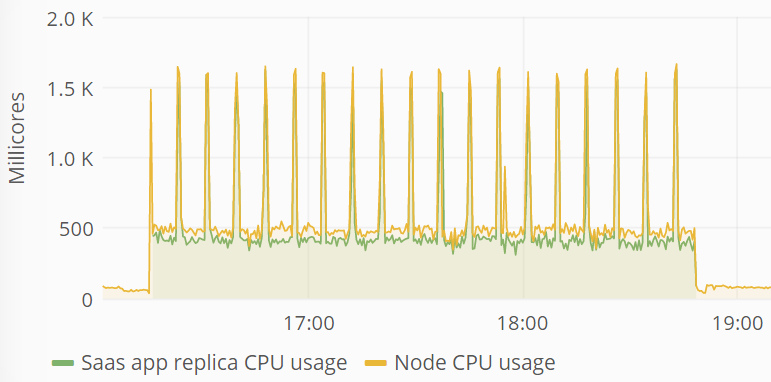
\includegraphics[width=0.70\columnwidth]{Images/Experiments/CPU/Grafana/cpu-saas-hpa-bursty-3-2.PNG}
\caption{Third worker node CPU usage.}
\label{fig:cpu-saas-hpa-bursty-3-2}
\end{subfigure}
\hfill
\vspace*{-7mm}
\caption{CPU usage during the second test of Experiment 6. Increasing the time between bursts to 7 minutes, replicas are not removed inbetween bursts, which is not as expected.}
\label{fig:cpu-saas-hpa-bursty-2}
\end{figure}

Neither these experimental results nor the official documentation about the HPA~\citep{hpa-algorithm-details} clarify how the HPA decides when to scale an application. Discovering the cause of this unexpected behavior is left for future work. The results show, however, that the HPA is unfit to process bursty workloads effectively.


\subsection{Experiment 7: Determining the effects of combining the Kubernetes HPA with the presence of a low priority pod}
Experiment 2 illustrated that co-locating a high and low priority pod has a minor impact on the high priority application's performance, while in increases the overall cost-efficiency. The goal of this experiment is to test whether this is still the case when the HPA is added to the cluster. 

\paragraph{Setup.}
The scaling point for the SaaS application is again set to 110\%. The application is subjected to the linearly increasing workload described earlier.


\paragraph{Results.}
Figure \ref{fig:lat-saas-li} shows the 95th percentile latencies recorded during this experiment. They are only slightly higher compared to the latencies recorded during Experiment 5. This slight decrease in performance again comes with the benefit of a higher resource utilization during low workloads, as illustrated by Figure \ref{fig:cpu-saas-lpp-hpa-li-1}. The low priority pod is able to use the excess of resources on the node during low workloads. As the workload rises, the low priority pod is given access to less CPU cycles. When a new replica of the SaaS application is added to the cluster, the amount of requests which the original replica needs to process lowers, again freeing up resources for the lower priority pod to use. 

%\begin{figure}
%\centering
%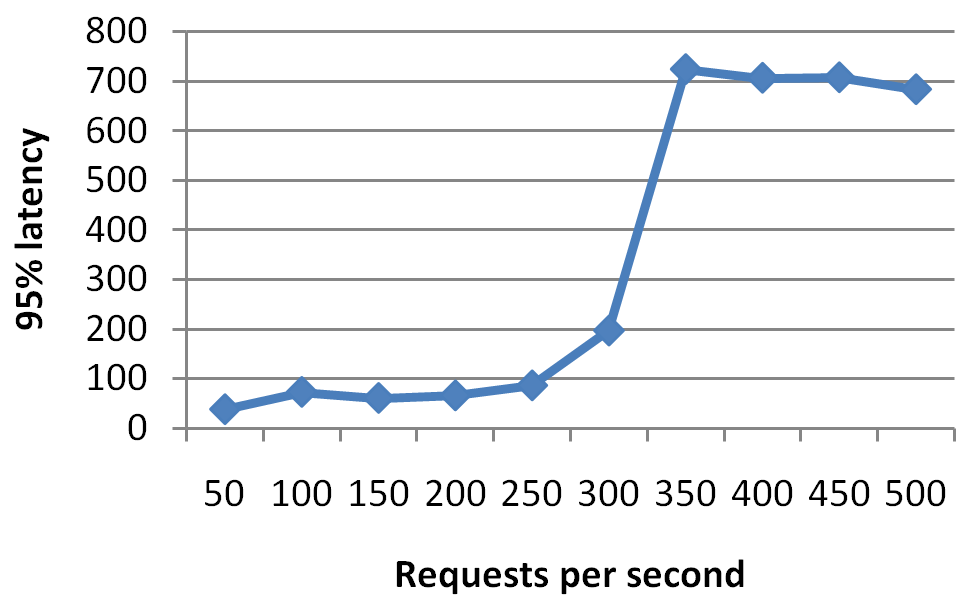
\includegraphics[width=0.60\columnwidth]{Images/Experiments/CPU/Latencies/lat-saas-lpp-hpa-li.PNG}
%\caption{95th percentile of latencies during experiment 7. They are only slightly higher than the ones recorded during Experiment 5. This indicates that adding a %co-locating a high and low priority pod increases cost-efficiency, even when the high priority pod is able to scale.}
%\label{fig:lat-saas-lpp-hpa-li}
%\end{figure}
%
%
\begin{figure}
\centering
\begin{subfigure}[b]{0.9\columnwidth}
\centering
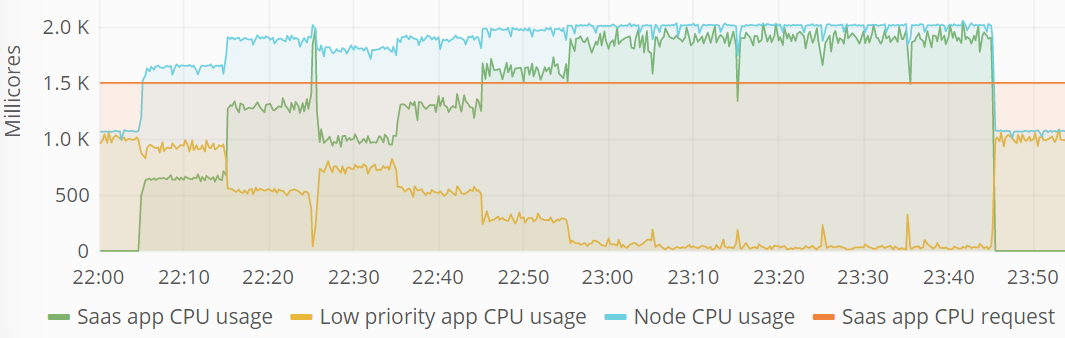
\includegraphics[width=0.75\columnwidth]{Images/Experiments/CPU/Grafana/cpu-saas-lpp-hpa-li-1.PNG}
\caption{First worker node's CPU usage.}
\label{fig:cpu-saas-lpp-hpa-li-1}
\end{subfigure}
\hfill
\begin{subfigure}[b]{0.9\columnwidth}
\centering
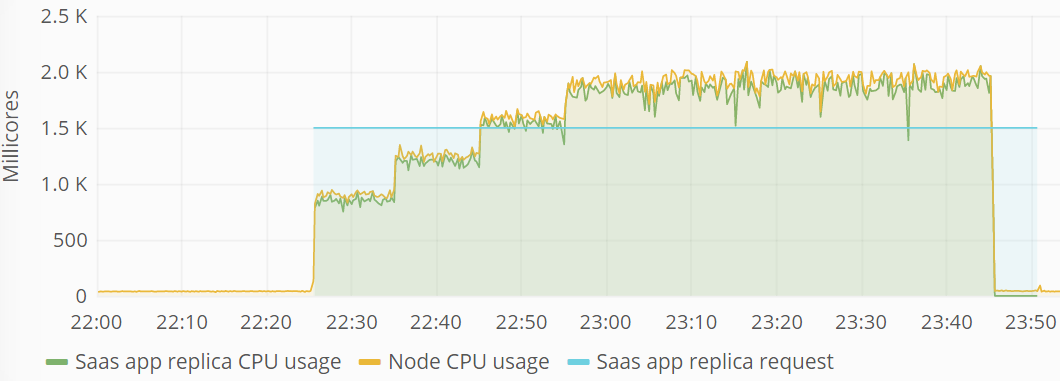
\includegraphics[width=0.75\columnwidth]{Images/Experiments/CPU/Grafana/cpu-saas-lpp-hpa-li-2.PNG}
\caption{First worker node's CPU usage.}
\label{fig:cpu-saas-lpp-hpa-li-2}
\end{subfigure}
\hfill
\vspace*{-3mm}
\caption{CPU usage during Experiment 7. A new replica is added when the scaling threshold is breached, and the freed up resources are made available to the low priority application.}
\label{fig:cpu-saas-lpp-hpa-li}
\end{figure}

\subsection{Threats to validity}
Some of the conclusions drawn from the experiments results may only be valid for the specific setup used in this paper. The performed experiments considered an environment with two user applications: one high priority application and one low priority application. Setting suitable requests and limits can, however, become a complex task if multiple pods with each different priorities are scheduled on the same node.

The type of test applications used can also impact the experiment results. The artificial SaaS application has a very short start-up time, making it well suited to be horizontally scaled. This may not be the case for other applications. Furthermore, this paper assumed that empty nodes were available for new replicas to be scheduled on. In practice, nodes may need to be acquired from IaaS providers and configured to the specific environment before they are ready to host applications. This could further increase the start-up time of new replicas. 

\section{Conclusion}
\label{chap:conclusion}
\subsection{Summary of findings}
This paper described the effects of different resource management mechanisms offered by Kubernetes, namely resource allocation via request and limit configurations and the Horizontal Pod Autoscaler. In environments with a small amount of applications and where low priority applications do not need any guarantees, experiments show that choosing proper request configurations increases cost-efficiency without major drawbacks. This was verified for a Cassandra based application and for an artificial SaaS application, as well as for both seasonal and bursty workloads. Due to an overhead introduced by running Cassandra on Kubernetes, scaling Cassandra in Kubernetes decreases performance instead of increasing it, regardless of the scaling algorithm used. The HPA performs well for an artificial SaaS application if the workload is seasonal, even if pods are co-located. For bursty workloads, other approaches may be preferred. In conclusion, despite some limitations, the scaling capabilities of Kubernetes show great potential to prevent SLA violations and increase resource cost-efficiency in container-centric environments.


% \paragraph{Request and limit configurations} 
% Experiments demonstrated that request and limit configurations greatly impact applications' performances on nodes with multiple pods. Allowing pods to use overprovisioned resources when needed effectively enables them to scale vertically without having to be rescheduled. A relatively high request gives pods a better claim to overprovisioned resources, and vice versa. Applications with a low request are allowed to use overprovisioned resources only if the other applications' workload is low. Co-locating low and high priority pods therefore increases cost-efficiency while only slightly impacting the performance of high priority applications, making the mechanism a useful tool for server consolidation purposes.

% These findings were confirmed for two applications: one Cassandra based log management service and one artificial SaaS-application. Moreover, the findings are valid for both seasonal and bursty workloads. The available resources are redivided almost instantly when there is a burst of workload. This makes the mechanism better suited to deal with bursty workloads than most horizontal scaling techniques, as starting new replicas is usually slow. 

% \paragraph{The Kubernetes HPA}
% Kubernetes introduces an overhead when running Cassandra. Experiments revealed that this overhead increases significantly as more replicas are added. This causes the performance of Cassandra to decrease rather than increase when scaling it in Kubernetes. The overhead is shown not to be caused by the HPA, but by Kubernetes itself. 

% For a seasonal workload, when scaling the artificial SaaS application using the HPA, only a minor overhead is observed. Scaling from one to two replicas causes the application's capacity to almost double. Furthermore, adding low priority pods to the node does not affect the operation of the HPA. The cost-efficiency benefit gained from setting adequate request configurations can thus also be leveraged when scaling applications using the HPA.

% With bursty workloads, experiments illustrated that using the default HPA leads to unexpected results. The HPA's scaling decisions are inconsistent: sometimes it decides to scale during a burst and sometimes it does not. At the time of writing, Kubernetes' official documentation concerning the HPA does not provide sufficient explanations for this behavior. 

% \subsection{Lessons Learned}
% Experiments illustrated that, in environments with a small amount of applications and where low priority applications do not need any guarantees, choosing proper request configurations increases cost-efficiency without major drawbacks. Due to an overhead introduced by running Cassandra on Kubernetes, scaling Cassandra in Kubernetes decreases performance instead of increasing it, regardless of the scaling algorithm used. The HPA performs well for an artificial SaaS application if the workload is seasonal. For bursty workloads or more complex environments, sophisticated approaches may be preferred. In conclusion, despite some limitations, the scaling capabilities of Kubernetes show great potential to prevent SLA violations and increase resource cost-efficiency in container-centric environments.
%
%\subsection{Future Work}
%A first possible extension to this paper is to further evaluate the HPA for bursty workloads. The cause of the HPA performing inconsistently could possibly be discovered by examining the exact scaling algorithm rather than the documentation. 
%
%A second extension could investigate the performance impact of scaling applications with a longer start-up time. In this case, the HPA may need to be configured differently to prevent SLA violations. Utilizing merely the HPA may not be sufficient to prevent SLA violations, however. Allowing high priority applications to use overprovisioned resources during scaling may prevent SLA violations when starting up a new replica is slow.
%
%A third possible extension could describe the effects of using the Kubernetes mechanisms when the workload is memory intensive. In this case, low priority pods get evicted instead of throttled. The performance impacts of request and limit configurations as well as scaling could be different. 



\bibliographystyle{plain}
\bibliography{references}

\end{document}

